\chapter[Capítulo 2]{Referencial teórico}

% Texto de abertura do capítulo. Substitua pelo seu conteúdo.
Texto introdutório do capítulo...

\section{2.1 Engenharia de Requisitos}

Texto da primeira seção...

\subsection{Subseção de exemplo}

Texto da subseção...

\section{Figuras e gráficos}

% Exemplo de inserção de figura. Ajuste o caminho e a legenda.
A Figura \ref{fig-cap2-01} apresenta...

\begin{figure}[h]
	\centering
	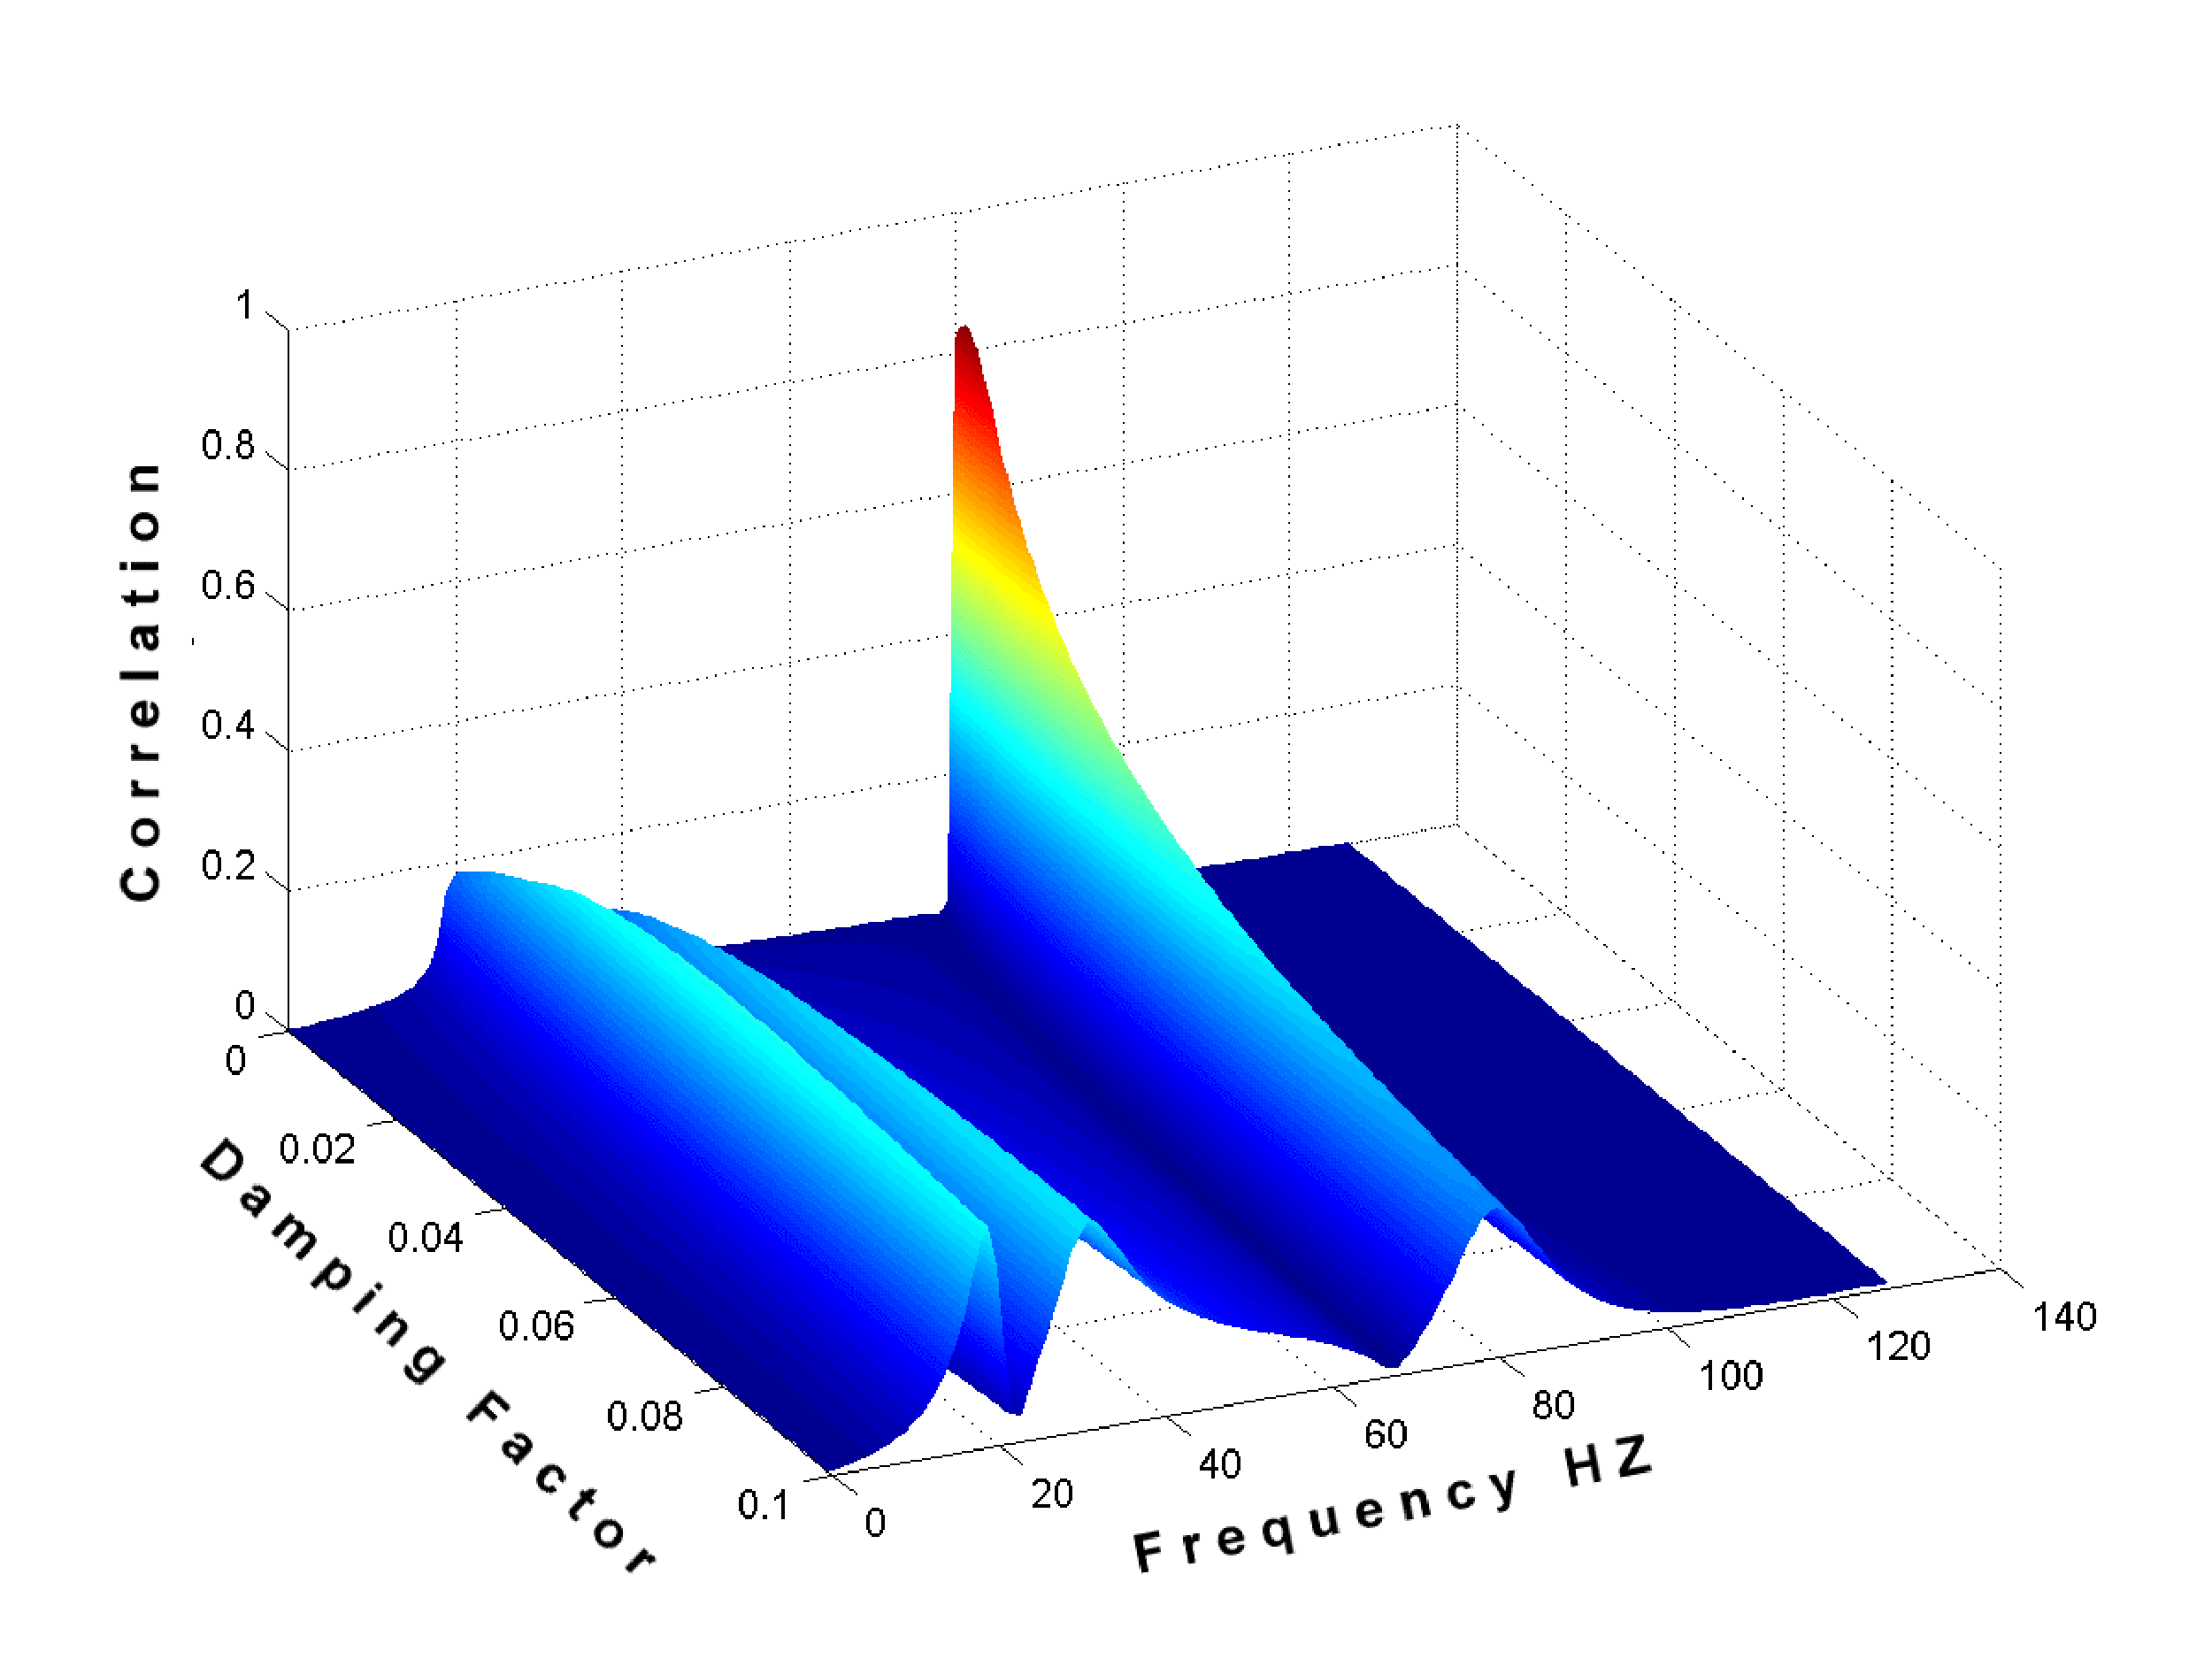
\includegraphics[keepaspectratio=true,scale=0.3]{figuras/fig01.pdf}
	\caption{Descrição da figura}
	\label{fig-cap2-01}
\end{figure}

\section{Tabelas}

% Exemplo de tabela. Ajuste colunas, dados e legenda.
A Tabela \ref{tab-cap2-01} resume...

\begin{table}[h]
	\centering
	\caption{Descrição da tabela}
	\label{tab-cap2-01}

	\begin{tabular}{ccc}
		\toprule
		\textbf{Coluna 1} & \textbf{Coluna 2} & \textbf{Coluna 3} \\
		\midrule
		Linha 1 & valor & valor \\
		Linha 2 & valor & valor \\
		\bottomrule
	\end{tabular}
\end{table}

\section{Equações}

% Exemplo de equação numerada.
Conforme a Eq. \ref{eqn-cap2-01},

\begin{equation}
	\label{eqn-cap2-01}
	y = a x + b.
\end{equation}

\section{Citações}

% Citação indireta e direta usando a bibliografia (bibliografia.bib).
Segundo \citeonline{Sommerville2007}, ...

\begin{citacao}
Trecho de citação direta com mais de três linhas, em fonte 10 e recuo de 4 cm \cite{Sommerville2007}.
\end{citacao}
